\documentclass[a4paper]{article}
\usepackage[T1]{fontenc}
\usepackage[utf8]{inputenc}
\usepackage[italian]{babel}
\usepackage{graphicx}

\begin{document}


\author{Lorenzo Casini \and Sophia Fantoni}
\title{PROGRAMMAZIONE DI RETI \\ REPORT ASSIGNMENT 1}
\maketitle

\newpage

\tableofcontents	%per fare l'indice

\newpage


\section{Task 1}

\subsection{Descrizione degli step}
Il primo passo che abbiamo eseguito per realizzare il primo task è la comprensione totale delle funzionalità di netcat. Digitando su terminale man nc è possibile leggere e comprendere le funzionalità che il comando ci mette a disposizione, digitando successivamente netcat (o nc) -h analizziamo solo le opzioni che ci interessa utilizzare. \\
Abbiamo deciso di sperimentare le funzionalità di netcat sia nel caso in cui Client e Server stiano sullo stesso host, sia nel caso in cui appartengano a due host diversi. \\


\subsection{Avvio dell'applicazione lato Client}
\paragraph{netcat -u localhost 1234	
		\\ nc -u 192.168.43.95 1234 \\ \\} 
Il primo scopo è quello di creare un Client mediante la suite nc.
Tra le opzioni scegliamo di specificare:
\par -u per dire esplicitamente di voler comunicare sfruttando il protocollo UDP, 
\par hostname: nel protocollo UDP è la stringa a 4byte che identifica l’indirizzo IP (localhost-> variabile riconosciuta da tutti, in alternativa avremmo potuto inserire l’indirizzo esplicito 127.0.0.1 Loopback sulla macchina locale, se voglio collegarmi ad una macchina remota inserisco l’IP del calcolatore).
\par port 1234: il numero di tale porta è scelta in modo arbitrario, l’unica cosa di cui bisogna preoccuparsi è che quella porta sia libera, è necessario non utilizzare le porte già assegnate ad altri protocolli (es. 80, 21, 22). \\ \\
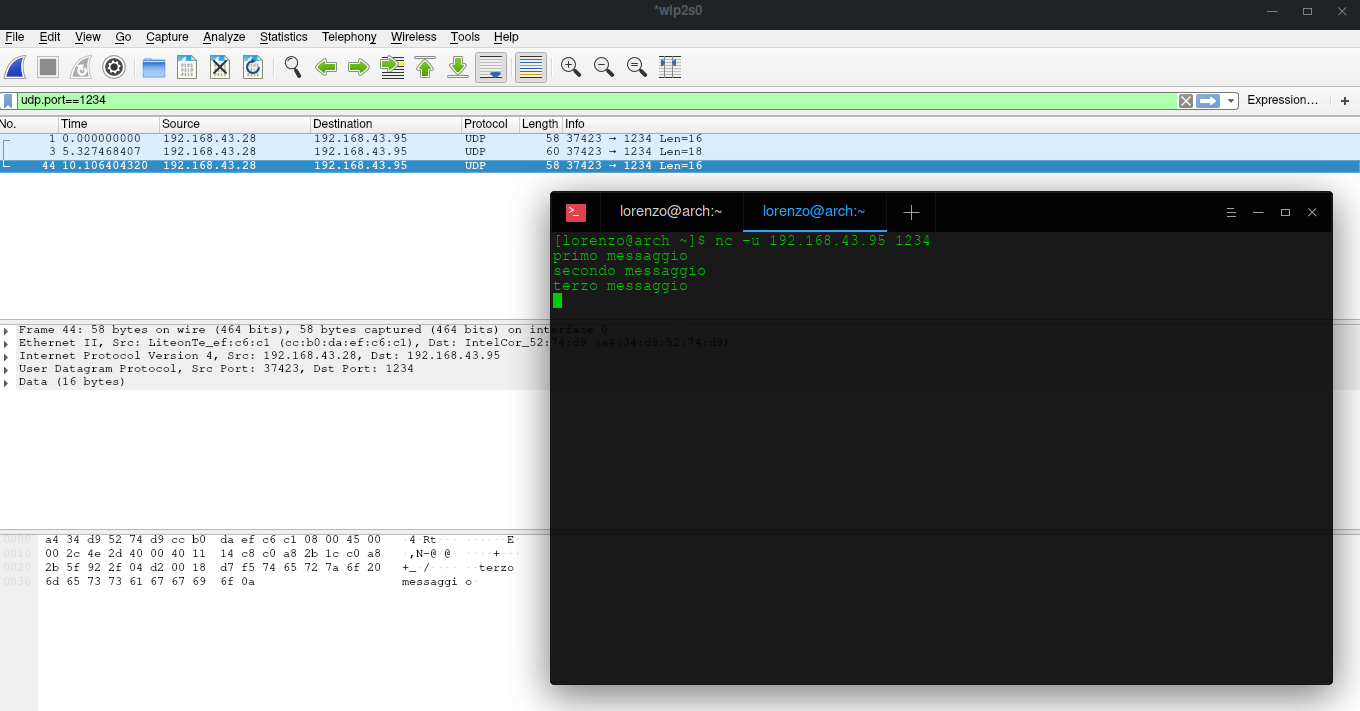
\includegraphics[width=\linewidth]{task_1/nc_client.png}

\newpage

\subsection{Avvio dell'applicazione lato Server}
\paragraph{netcat -u -l 1234 \\}
Successivamente istanziamo il Server, in questo caso non dobbiamo specificare l’hostname, per questo motivo non dovremo variare la riga di comando nel caso in cui gli host appartengano allo stesso o a due host differenti.
\par -u per far in modo che ascolti solo i pacchetti di tipo UDP.
\par -l per dire che deve ascoltare (listen) qualsiasi connessione (inviato da un qualsiasi host) in entrata.
\par 1234 è la porta su cui deve mettersi in ascolto.

\par Per analizzare il traffico che viene generato dalla loro connessione utilizziamo Wireshark.
\par Nel primo caso, quello in cui il Server e il Client appartengano allo stesso host, mi metto in ascolto sull’interfaccia di Loopback, e avvio la cattura dei pacchetti. Nel secondo filtro solo i dati che passano sull’interfaccia enp0s3. \\ Per prendere effettivamente il solo traffico che client e server si scambiano sulla porta 1234 con protocollo UDP devo inserire dei filtri. udp.port==1234 tale filtro mi permette di escludere tutte le connessioni che non siano locali di tipo UDP che girano sulla porta 1234. 
\par Il client invia il pacchetto dalla porta 37423, tale porta viene scelta in modo arbitrario al momento dell’apertura del client; se eseguo uno stesso client più volte tale porta può cambiare. \\ \\

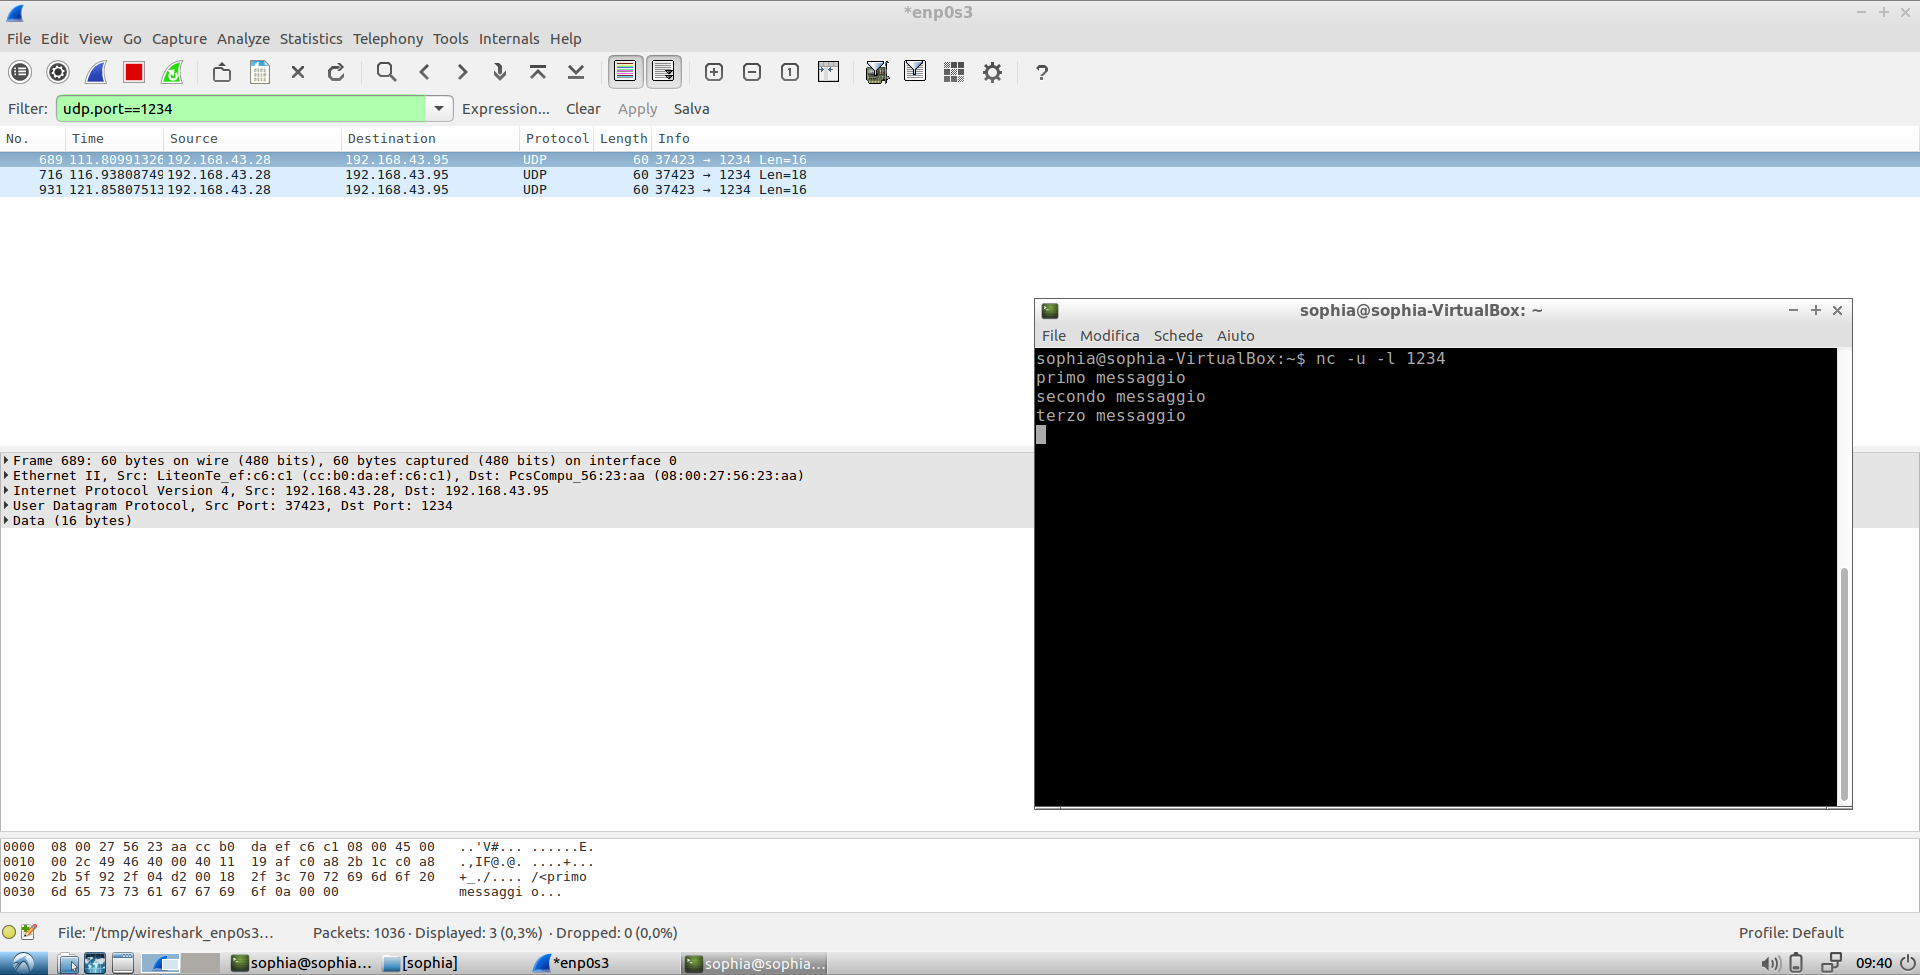
\includegraphics[width=\linewidth]{task_1/nc_server.png}
\newpage
\subsection{Note sul funzionamento di netcat}
Dai test effettuati (utilizzando i nostri comandi) con netcat abbiamo compreso il suo funzionamento. Per quanto riguarda la parte UDP abbiamo notato che una volta che un Client invia un pacchetto al Server, quest’ultimo rimane in ascolto solo dei pacchetti ricevuti da quel specifico client, perciò altri client vengono ignorati. Quando terminiamo l’esecuzione del client specifico è necessario terminare anche il server in quanto esso non è in grado di accettare pacchetti da altri client. Infine, una volta instaurata la connessione, appare chiaro che netcat non distingue lato client dal lato server, inquanto è possibile inviare messaggi anche dal Server verso il Client.
\\

\section{Task 2}
\subsection{Strategia di risoluzione client/server}
Per realizzare il secondo task è stato necessario innanzitutto comprendere le funzionalità di nc, ciò è stato immediato dopo la realizzazione del task 1, e successivamente analizzare e modificare il codice consegnatoci durante le ore di laboratorio. 

\subsection{Comportamento dettagliato client/server}
Il Client e il Server, per poter essere avviati, necessitano l’inserimento in input dell’indirizzo IP e del numero di porta. Il Server per poter inviare una risposta al Client, estrae da ogni datagramma ricevuto l’indirizzo IP e il numero di porta del mittente. 
\par Il file udpclient.c crea la socket con i parametri presi al momento dell'avvio (IP\_SERVER, PORTA).\par Il Client è in grado di inviare messaggi al Server, nel caso in cui la stringa inviata dal Client coincida con "exit", esso si metterà in attesa della risposta da parte del Server, se tale risposta risulta essere  “Goodbye” la socket verrà chiusa. 
\par Il Server crea la socket, legge i datagram ricevuti, controlla se contengono la stringa “exit”, in tal caso invia come risposta al Client la stringa “Goodbye”, altrimenti rimane in attesa di ulteriori messaggi. Il Server dopo la richiesta di chiusara della connnessione da parte del Client, rimane in esecuzione e non  chiude la propria socket.
\newpage
\subsection{Test}
Abbiamo sperimentato il codice avviando Client e Server su due host differenti.\par
\begin{flushleft}
\textbf{client:}
\end{flushleft}
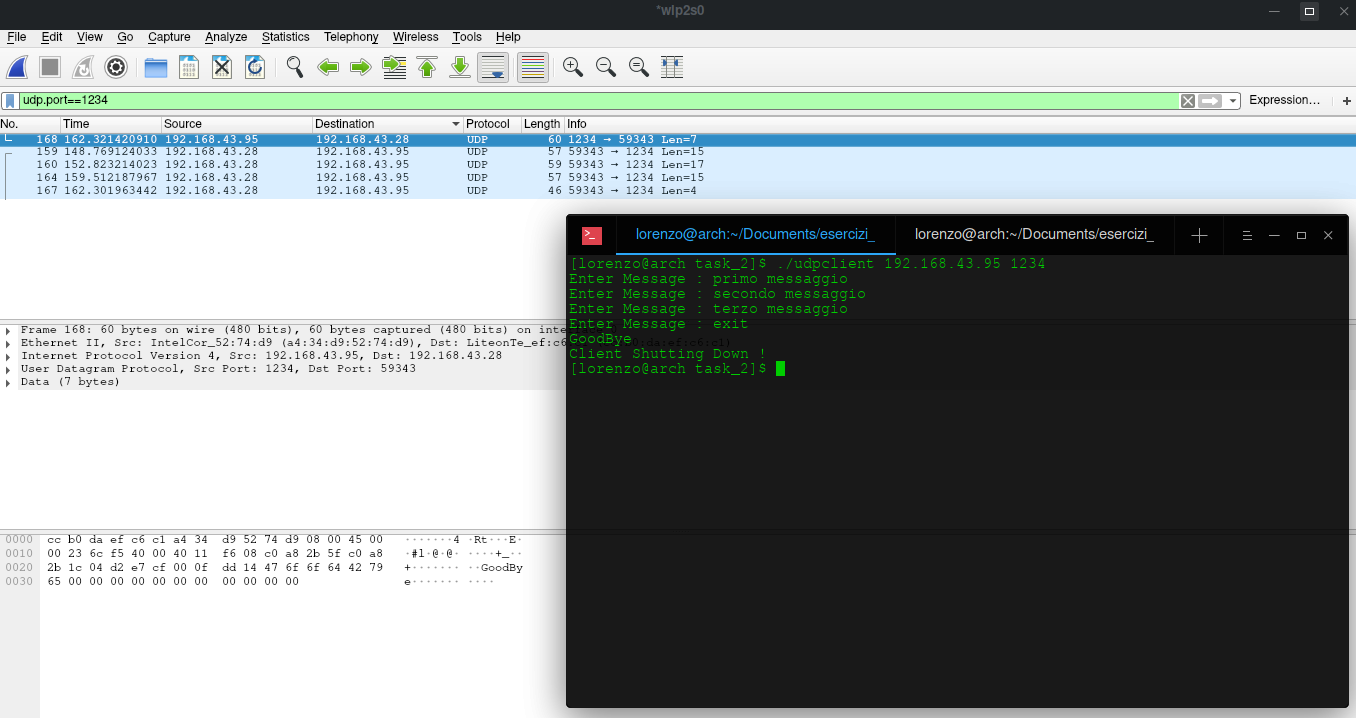
\includegraphics[width=\linewidth]{task_2/udp_client.png}
\begin{flushleft}
\textbf{server:}
\end{flushleft}
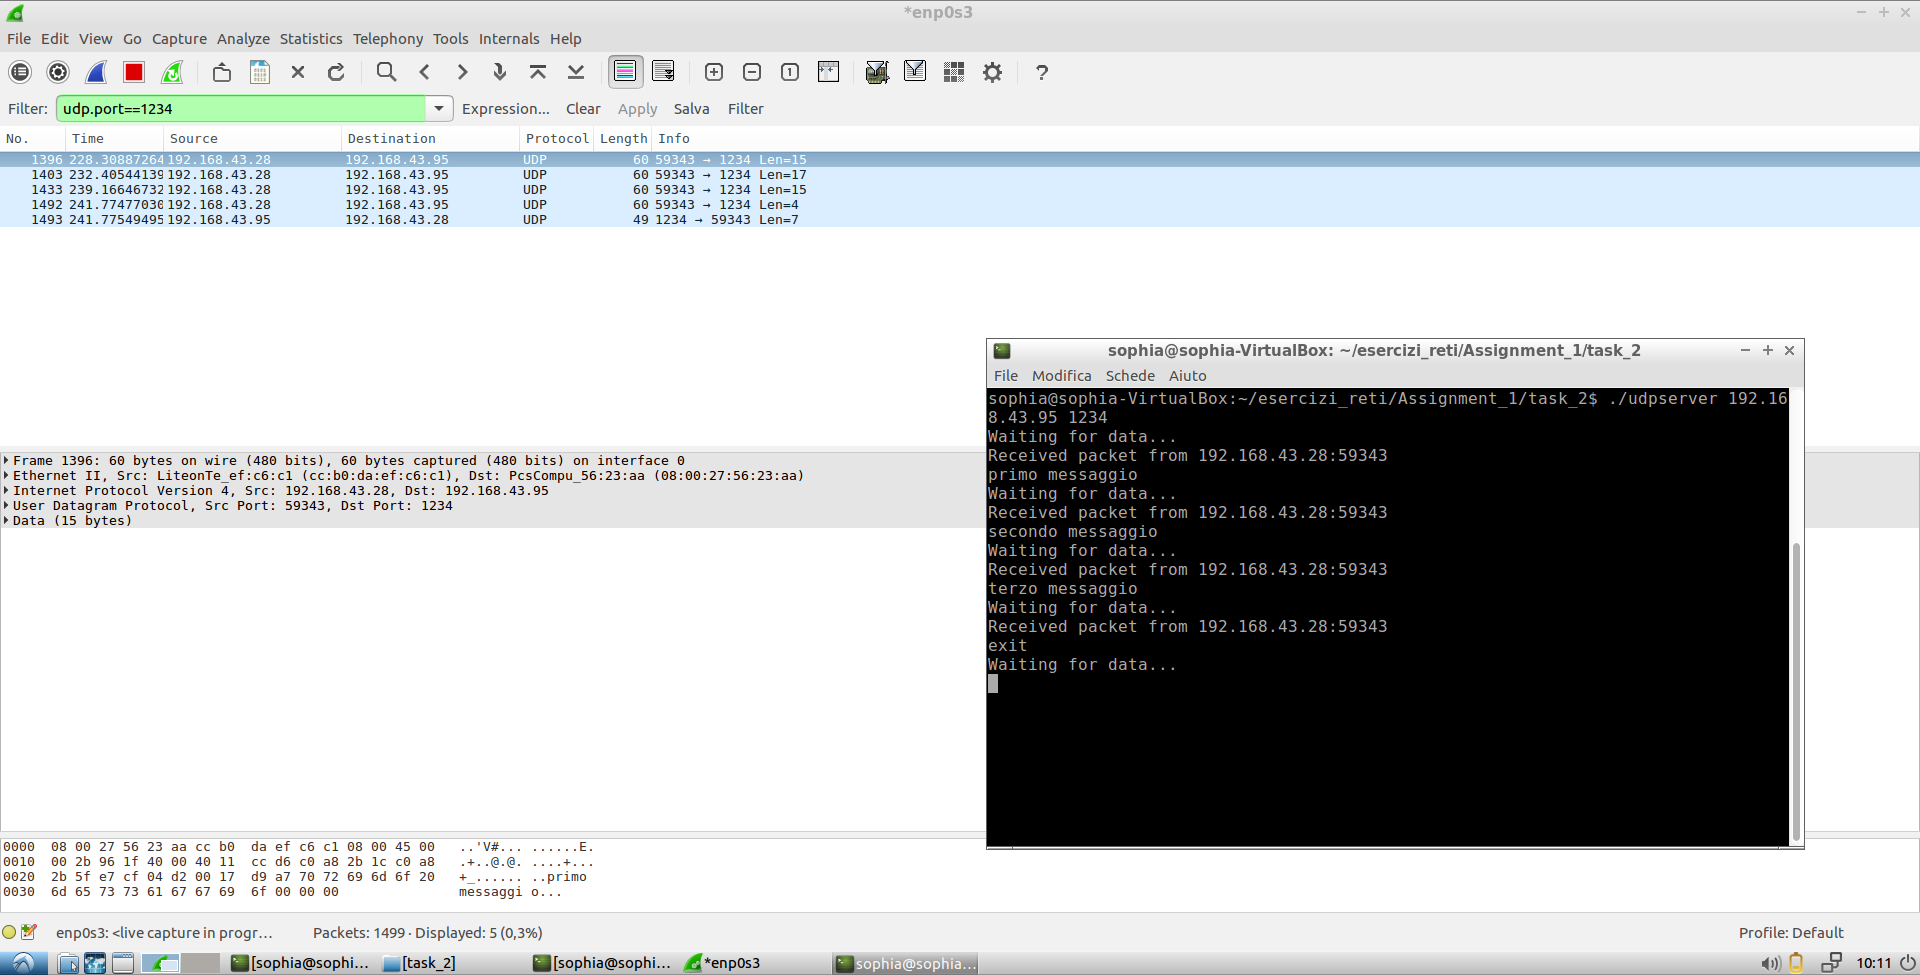
\includegraphics[width=\linewidth]{task_2/udp_server.png}

\newpage

\section{Task 3}
\subsection{Risposte alle domande}
Per effettuare il terzo task abbiamo utilizzato il codice scritto da noi e utilizzato nel task 2. Avviando due client che comunicano con lo stesso server, le operazioni svolte dal server sembrerebbero concorrenti perché le poche operazioni che esegue impiegano un lasso di tempo molto breve. \\ 
Successivamente, per simulare operazioni più complesse, decidiamo di inserire una sleep prima della funzione recivefrom. Questa operazione risulta più impegnativa dal punto di vista del tempo all’interno del codice. Eseguendo questa prova abbiamo osservato che il protocollo esegue in realtà le operazioni in modo sequenziale, in quanto queste vengono eseguite, quindi stampate a video, intervallate dal periodo di tempo della sleep inserita.

\subsection{Motivazioni}
\par Avendo implementato il server senza l’utilizzo di thread, esso è in grado di gestire un pacchetto alla volta completando le operazioni richieste.
\par Una volta completate tali operazioni il Server sarà in grado di ricevere un nuovo pacchetto e riavviare le operazioni su di esso. 
\par Quindi, per ottenere un comportamento concorrente, è necessario creare lato server un thread in grado di gestire tutte le richieste in ingresso. Esso si preoccuperà di creare un nuovo thread per ogni nuova connessione richiesta. Il server effettua un controllo su ogni pacchetto, verificandone  ip e porta e lo inoltrerà al thread che sta gestendo tale connessione, in caso il thread non esista verrà creato. Ovviamente questa tipo di gestione implica che il numero di connessioni accettate dal server venga controllato e/o limitato per evitare di incorrere in vari tipi di errori. 


\end{document}